\fdocabbrevdeclare{KDE}{KDE}{K Desktop Environment}
\chapter{Foreword}
Qt framework \citep{various:qthome} is one of the greatest libraries ever made. You probably use it and you don't even know about it. If you use Skype\index{Skype} \citep{various:skype} or \fdocabbrevref{KDE}\index{KDE} \citep{various:kde}, then you use Qt too, because those applications are based on Qt.

Skype uses just graphical interface made in Qt but \fdocabbrevref{KDE} is totally based on Qt as it uses not just graphical interface from Qt but other components too.

Qt penetrated the world of interactive applications and now it can be found even in devices, where it's not generally expected. First public version of Qt was released in 1995 and huge progress was achieved since that time.

In a matter of time, Qt began to be perceived as very dynamic library which is particularly great for graphical interface design. There was very good reason for such an opinions because \fdocabbrevref{KDE} was released in 1996, invoking quite a sensation. In short, its desktop environment looked great and overpowered other major environments in this aspect. Qt was pushed forward by those events and became massively popular. The only goal of Qt was to be a good library for anyone who does desktop programming.

As years passed, Qt was more and more robust, \fdocabbrevref{KDE} made its progress through version 3 and 4, and things have changed. Presently, desktop\index{desktop} does not mean everything for application developer. Today cyber-world needs to be interconnected and people want to be mobile. You can't do that with desktop environment running on personal computer. You need cell-phone. Cell-phone with (possibly) good-looking environment and fancy applications. Unfortunately, Qt 4 was not able to offer this kind of functionality to its users\,--\,programmers, so they looked at the competition and chose Android\index{Android} as their platform, leaving Qt behind.

Luckily, Qt 5 appeared, bringing us some new exciting features, giving itself a chance to compete its opponents in category of mobile development toolkits. If we add rock-solid desktop features, we have versatile and stable base to build on.

\vfill

\section{What is Qt?}\label{section:what}
As said previously, Qt is framework, toolkit or, simply, set of libraries. It has its very roots in Norway. Original creators are Haavard Nord\index{Haavard Nord} and Eirik Chambe-Eng\index{Eirik Chambe-Eng}. \citep[section History]{various:qtwikip} Basically Qt framework consists of:
\begin{itemize}
\item set of libraries written in \cpp,
\item meta-object compiler\index{meta-object compiler},
\item QtScript interpreter\index{QtScript},
\item tools for internationalization\index{internationalization} and \fdocabbrevref{GUI} design,
\item scripts for various build systems like CMake\index{CMake},
\item other tools, \eg integrated development environment, examples or documentation browser.
\end{itemize}

So as you see, Qt is not just collection of header/source files. It's completed with a variety of other stuff. You will learn more about Qt structure in \autoref{section:qtstructure}.

\section{Companies behind Qt}
Qt lives for more than two decades and its owners changed accordingly. Haavard Nord and Eirik Chambe-Eng assembled themselves in a team and called it Quasar Technologies. Later company was renamed to Trolltech. This company led Qt development for period of 12 years, preffering desktop development.

\fdocabbrevdeclare{POSIX}{POSIX}{Portable Operating System Interface}

But as we know, things have changed and smartphones became massively popular in third millennium. That's why Trolltech was acquired by Nokia. It was obvious that Nokia can bring something new to Qt as it is leading company in smartphones world production. Nokia promised that they would keep Qt open-souce and made it available via public Git\footnote{Git is revision control system originally created to support Linux kernel development. Founding author is well-know Linus Torvalds\index{Linus Torvalds}. Git is multi-platform and is available for Windows, Linux or Mac OS X. It's \fdocabbrevref{POSIX}-compatible.}\index{Git} repository. Nokia somehow was not able to utilize potential of Qt and sold it to another company called Digia. \citep{various:qtwikip}

\subsection{Licensing}
Qt uses two separate licenses:
\begin{enumerate}
\item \textbf{Commercial license}, which provides you (as indie developer) with opportunity to produce \textit{closed-source} (proprietary) or \textit{open-source} applications, you can do whatever you want with your copy of Qt. This kind of license is usually sold per particular platform and it is generally rather expensive. This license is usually bought by developers who want to sell their software and/or keep it closed-source, otherwise open-source license is better choice.

Commercial license grants you even more rights. You can link Qt statically to your application and/or include other proprietary software in it. Technical support is available for commercial users only.

\item \textbf{Open-source license}, which provides you (and your users) with much more freedom but forcing you to share source code of your application with the community and allowing anyone to change your application and redistribute it under the same terms. Used license is GNU LGPL\index{licenses!GNU LGPL} license, in version 2.1, and GNU GPL\index{licenses!GNU GPL} \citep{stallman:gnugpl} for your projects.
\end{enumerate}

Licenses have always been quite a problem to Qt framework. Commercial license was fine. However, non-commercial was not. Qt used its own license before GNU LGPL and GNU GPL were chosen as primary ones. Problem was that Q Public License\index{Q Public License} wasn't GPL compatible. This problem became much more obvious when \fdocabbrevref{KDE} established itself as one the most favored desktop environments, gaining milions of users. They were naturally afraid of KDE becoming the piece of proprietary software, which was more or less possible with Q Public License. Luckily this problem was solved by releasing Qt under GNU GPL.

\fdocabbrevdeclare{OOP}{OOP}{Object-oriented programming}
\section{C plus plus as base stone}\label{subsection:cpp}
\cpp{} is known as general-purpose programming language, based on C. It was created around 1979 by Bjarne Stroustrup\index{Bjarne Stroustrup}, bringing in many \fdocabbrevref{OOP} features such as implementation of classes, polymorphism, entity overloading or inheritance. You can find brief example of basic techniques in \autoref{listing:sampleoop}.

\begin{fdoccode}{cpp}{listing:sampleoop}{Basic \fdocabbrevref{OOP} techniques in \cpp}
/* Base class declaration */
class BaseClass {
    public:
		BaseClass() {
		    cout << "BaseClass instance constructed." << endl;
		}

		void BaseClass::whoAmI() const {
		    cout << "I am BaseClass." << endl;
		}
};

/*
 * Class declaration
 * This class inherits BaseClass.
 */
class InheritingClass : public BaseClass {
	public:
		InheritingClass() : BaseClass() {
		    cout << "InheritingClass instance constructed." << endl;
		}
		
		void InheritingClass::whoAmI() const {
		    cout << "I am InheritingClass." << endl;
		}
};

/* Usage of BaseClass and InheritingClass classes. */
int main() {
    BaseClass class_1;
    InheritingClass class_2;
    class_1.whoAmI();
    class_2.whoAmI();

    BaseClass *class_3 = &class_2;
    class_3->whoAmI();

    ((InheritingClass*) class_3)->whoAmI();

    return 0;
}
\end{fdoccode}

\begin{fdoccode}{text}{}{Output of application from \autoref{listing:sampleoop}}
BaseClass instance constructed.
BaseClass instance constructed.
InheritingClass instance constructed.
I am BaseClass.
I am InheritingClass.
I am BaseClass.
I am InheritingClass.
\end{fdoccode}

\cpp{} has many characteristics\,--\,some are bad while other ones may be great.
\begin{description}
\item[SYNTAX\ts{\textcolor{red}{bad}}]\hfill \\
\cpp{} is known to have some oddities rooted in its syntax, \eg we can be confused by rife usages of\fdocinlinecode{cpp}{!}{const} keyword. One\fdocinlinecode{cpp}{!}{const} marks methods which can operate only with constant objects and another distinguishes constant variables from non-constant ones. Even the greatest fan of \cpp{} has to admit uncomfortable usage of this keyword. You can read about this topic in \citep[p.~90--92, p.~537]{prata:cprimer}.

\item[POINTERS vs. REFERENCES\ts{\textcolor{red}{bad}}]\hfill \\
This could be one of conventions-related issues. Programmers are not entirely sure whether to use pointers\index{pointer} or references\index{reference} for passing values to functions. Generally, terms of references and pointers usage are not strictly set.

\item[MEMORY MANAGEMENT\ts{\textcolor{red}{bad}, \textcolor{ultragreen}{good}}]\hfill \\
This is very discussed topic these years as many programmers transitioned to programming languages which produce
\emph{managed code}\index{managed code} (see explanation below). Nowadays programmers heavily depend on managed code and they have troubles with manual
object deletion and other related actions.

\begin{fdocextra}
Term \textit{managed code} means that all resources (usually called \emph{objects} in the object-oriented programming) generated by code execution are maintained and managed by an external entity. This entity is often called \emph{a virtual machine}\index{virtual machine} and usually includes sophisticated garbage collector, which is responsible for freeing needless resources from memory.
\end{fdocextra}

\cpp{} is considered to be a fairly low-level programming language. Its \enquote{\textit{low-levelness}} applies to the way the memory is managed. In this case, no automatic memory management is implemented, yielding responsibility to the programmer. He has to take care of memory allocation and deallocation. There is certainly quite big pronenes to errors in this approach. Programmers simply forgets to free allocated memory space and memory leak\index{memory leak} occurs.

On the other, manual management of allocated objects gives programmer bigger power to control application memory usage and that's perfect on devices with limited system memory. Manual control of object life can be also much faster than automatic resource management provided by \textit{garbage collectors}\index{garbage collector}.

Neither virtual machine nor complex runtime environment supports execution of \cpp{} application, thus \enquote{nobody} supervises actions of your application, except operating system. Your application is left alone with its segment of primary memory and your application is entrusted with everything, including memory management.

\item[THREADING\ts{\textcolor{red}{bad}}]\hfill \\
\cpp{} doesn't contain unified interface for threading.\footnote{Threading is supported in new \cpp{} 11 standard. You can read about threading\index{threading} inclusion in \citep[p.~1114-1160]{various:cppstandard}.} That could make pure \cpp{} poorly usable for developing more complex applications if no \nth{3}-party threading library is available.

\item[FAST CODE EXECUTION\ts{\textcolor{YellowOrange}{great}}]\hfill \\
\cpp{} code execution is amazingly fast compared to other modern programming languages. Direct compilation (see more in \autoref{section:compilation})  into machine code is the cause here. Other favorite languages are compiled into bytecode, thus they have to be compiled just-in-time by virtual machine and that is time consuming job, thus making application execution slow.

\fdocabbrevdeclare{IL}{IL}{Intermediate Language}
Let's make a little test and compare \cpp{} with \csharp. \csharp{} code is known to be compiled into \fdocabbrevref{IL}, which is bytecode, and ran by special runtime.

One of the simplest tasks to compare these two languages could be simple integer array sorting. Quicksort algorithm will do that. Consider implementations in \cpp{} (\autoref{listing:quickcpp}) and \csharp{} (\autoref{listing:quickcsharp}). Furthermore, we can use try to maximally optimize \csharp{} code execution speed by allowing \enquote{unsafe code} and using pointers instead of references. This approach is shown in \autoref{listing:quickcsharp-unsafe}.

Series of sample sortings was made with each implementation. Subject of sorting was array filled with descending integers. Such an array can be denoted as $Array = \left\{ x, x-1, x-2, \ldots, 0 \right\}$. Series contains 20 these arrays. Results of comparison are displayed in \autoref{figure:comparison}.

\begin{fdoccode}{cpp}{listing:quickcpp}{Quicksort implementation in \cpp}
void QuickSort::quickSort(int *array, int p, int r) {
    int q;
    if (p < r) {
		q = partition(array, p, r);
		quickSort(array, p, q - 1);
		quickSort(array, q + 1, r);
    }
}

int QuickSort::partition(int *array, int p, int r) {
    int x = array[r];
    int i = p - 1;
    int j;
    for (j = p; j < r; j++) {
		if (array[j] <= x) {
	    	i += 1;
	    	swap(&array[i], &array[j]);
		}
    }
    swap(&array[i + 1], &array[r]);
    return i + 1;
}

void QuickSort::swap(int *lhs, int *rhs) {
    int temp = *lhs;
    *lhs = *rhs;
    *rhs = temp;
}
\end{fdoccode}

\begin{fdoccode}{csharp}{listing:quickcsharp}{Quicksort implementation in \csharp}
static void quickSort(int[] array, int p, int r) {
	int q;
	if (p < r) {
		q = partition(array, p, r);
		quickSort(array, p, q - 1);
		quickSort(array, q + 1, r);
	}
}

static int partition(int[] array, int p, int r) {
	int x = array[r];
	int i = p - 1;
	int j;
	for (j = p; j < r; j++) {
		if (array[j] <= x) {
			i += 1;
			swap(ref array[i], ref array[j]);
		}
	}
	swap(ref array[i + 1], ref array[r]);
	return i + 1;
}

static void swap(ref int lhs, ref int rhs) {
	int temp = lhs;
	lhs = rhs;
	rhs = temp;
}
\end{fdoccode}

\begin{fdoccode}{csharp}{listing:quickcsharp-unsafe}{Quicksort implementation in \enquote{unsafe} \csharp}
static unsafe void quickSort(int* array, int p, int r) {
	int q;
	if (p < r) {
		q = partition(array, p, r);
		quickSort(array, p, q - 1);
		quickSort(array, q + 1, r);
	}
}

static unsafe int partition(int* array, int p, int r) {
	int x = array[r];
	int i = p - 1;
	int j;
	for (j = p; j < r; j++) {
		if (array[j] <= x) {
			i += 1;
			swap(&array[i], &array[j]);
		}
	}
	swap(&array[i + 1], &array[r]);
	return i + 1;
}

static unsafe void swap(int* lhs, int* rhs) {
	int* temp = lhs;
	lhs = rhs;
	rhs = temp;
}
\end{fdoccode}

\begin{figure}[ht]
\centering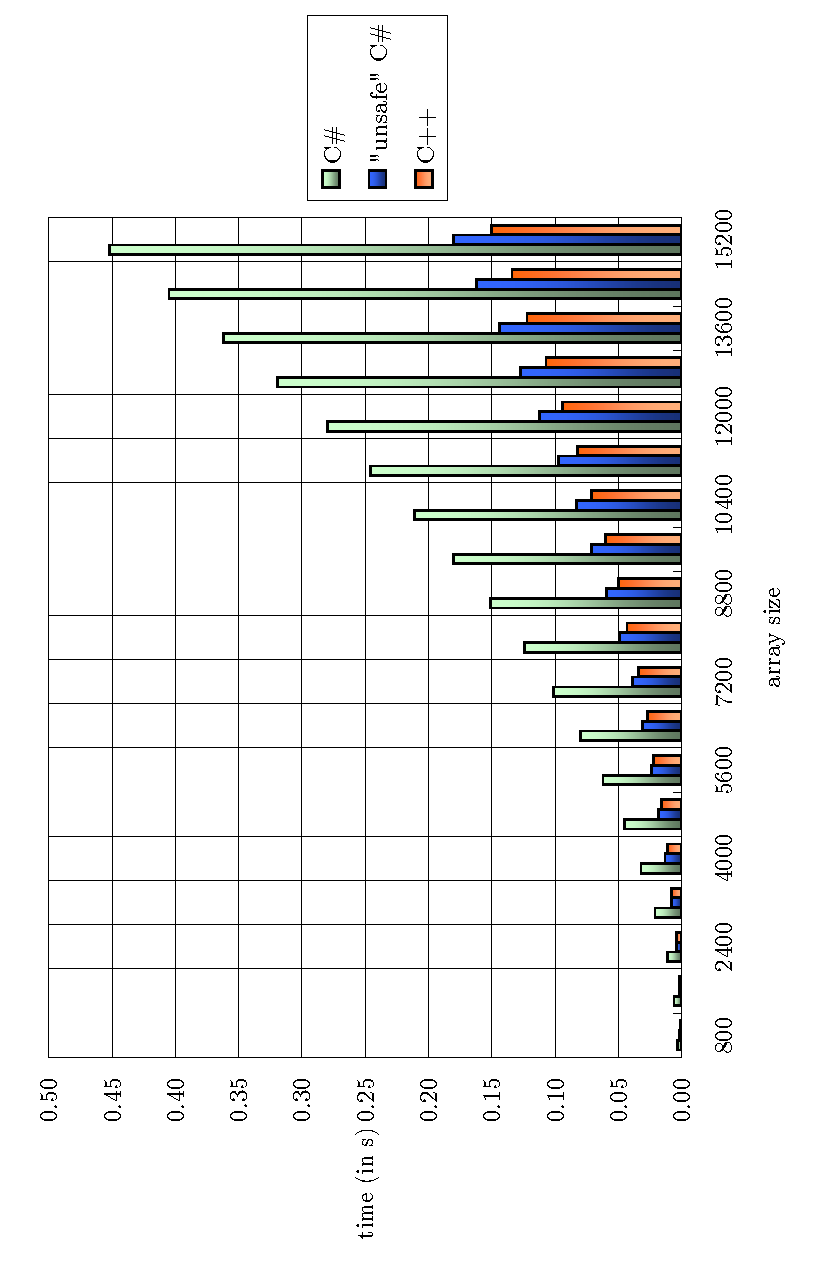
\includegraphics[width=9cm,angle=-90]{graphics/laboratory/00-langcomparison.pdf}
\caption{\cpp{} vs. \csharp{} comparison\,--\,Quicksort algorithm}\label{figure:comparison}
\end{figure}

We can see that \cpp{} outperformed classic \csharp{} implementation, while being aproximately 3 times faster. Even \enquote{unsafe} \csharp{} implementation got beaten, although the difference was tiny. So we can state that \cpp{} is faster than \csharp{} even in fairly simple task. You may think about performance difference if hugely complex computation (\eg rendering of 3D scene) is needed to be done.

\item[HUGE COMMUNITY\ts{\textcolor{YellowOrange}{great}}]\hfill \\
Plenty of world-renowned software is written using \cpp{}, including many 3D games, almost all programs from Adobe as well as Chromium web browser. Many \cpp{} books are available, which makes it easier to learn.

\vfill

\fdocabbrevdeclare{JRE}{JRE}{Java Runtime Environment}
\item[MEMORY CONSUMPTION\ts{\textcolor{ultragreen}{good}}]\hfill \\
\cpp{} applications, as stated, need no virtual machine for their execution. They just load standard \cpp{} library and extra libraries if needed. Such approach is significantly different from robust and memory greedy runtime environments of some high-level languages. We can mention particularly .NET Framework and \fdocabbrevref{JRE}.

\item[CODE PORTABILITY\ts{\textcolor{red}{bad}}]\hfill \\
When it comes to \textit{code portability} (which is just another term for \textit{multi-platformity}), \cpp{} leaves its users uncertain. They can be sure about portability of \cpp{} standard library but that's all. Standard library is not trully packed with stunning features, forcing you to use \nth{3}-party libraries for advanced functionality. Those libraries don't have to be multi-platform, which can be problematic if you want to port your application to another platform.

\item[MISSING CONSTRUCTS\ts{\textcolor{red}{bad}}]\hfill \\
Indeed, \cpp{} might be missing some very useful language constructs, which are quite common in other (\eg functional, logic or even declarative) programming paradigms. Many features emerged in \cpp{} 11 revision, however.
\end{description}

\vfill

\subsection{Version 11 and its enhancements}
\cpp{} programming language was standardized in 1998. This version is known as \cpp{} 98 and if someone talks about \cpp, he probably has this version in mind. Programming was changing in time. So, \cpp{} had to change to catch new trends and demands of its users.

\cpp{} 11 brought many new features, eliminating some of its annoyances. You can read about \cpp{} 11 in \citep{various:cppstandard} or go through its finest new properties right now. It is recommended to know something about \cpp{} 11 because Qt 5 uses its enhancements on some compilers.

\subsubsection{Basic C plus plus 11 information}
\cpp{} 11 is source code compatible with C and with \cpp{} 98. It means that valid C (or \cpp{} 98) source code is valid \cpp{} 11 code too. Inprovements in \cpp{} were done in two categories: language core and standard library.

\paragraph{Language core improvements}
Syntax of \cpp{} was always considered to be bad, which is partially true, because \cpp{} offers huge collection of syntactical constructs and sugar, compared to other well-known programming languages. Moreover, \cpp{} 11 adds new language constructs.

\paragraph*{Compile time constants}
In \cpp{} 98, you cannot write this piece of code:
\begin{lstlisting}[firstnumber=1,language=cpp]
int happy_number() {
	return 7;
}
int *array = new array[10];
array[happy_number()] = happy_number();
\end{lstlisting}
In this case, compilation ends with error saying: \enquote{Function \fdocinlinecode{cpp}{!}{happy_number()} is not a constant expression.} But you think it is. It returns $7$ everytime it's called, so it actually is constant expression. That's true but compiler is not aware of it. Keyword\fdocinlinecode{cpp}{!}{constexpr} tells the compiler to regard\fdocinlinecode{cpp}{!}{happy_number()} as constant expression, resulting in this code:
\begin{lstlisting}[firstnumber=1,language=cpp]
constexpr int happy_number() {
	return 7;
}
int *array = new array[10];
array[happy_number()] = happy_number();
\end{lstlisting}

\paragraph*{Initializer lists}
Consider the custom class which encapsulates\fdocinlinecode{cpp}{!}{std::list} and perhaps adds some functionality:
\begin{lstlisting}[firstnumber=1,language=cpp]
class CustomList {
	private:
		std::list<int> m_list;
	
	public:
		CustomList() { }
		
		void insert(int i) {
			m_list.push_back(i);		
		}
};
\end{lstlisting}
Such an implementation allows you to instantiate empty\fdocinlinecode{cpp}{!}{CustomList} and fill it with values one by one via\fdocinlinecode{cpp}{!}{insert(int i)} method. What if you know all values in compile time? In older \cpp{} you would have to insert all values one by one.

It would be nice if one could use better syntax for constructing\fdocinlinecode{cpp}{!}{CustomList} instances, array brace initializer syntax would be great. Its example usage looks like this:\fdocinlinecode{cpp}{!}{CustomList my_list_instance =  \{1, 2, 3, 4, 5, 6, 7\};}.

\cpp{} 11 allows you to use this syntax via initializer list:
\begin{fdoccode}{cpp}{listing:initializer}{Initializer list usage}
class CustomList {
	private:
		std::list<int> m_list;
	
	public:
		CustomList() { }
		CustomList(std::initializer_list<int> values) {
			for (int &value : values) {(*@\label{listing:forloop}@*)
				m_list.push_back(value);			
			}
		}
		
		void insert(int i) {
			m_list.push_back(i);		
		}
};

// Creating CustomList instance and filling it with values.
CustomList my_list_instance = {1, 2, 3, 4, 5, 6, 7};
\end{fdoccode}

\paragraph*{Clever for-loops}
Careful reader certainly noticed strange notation of for-loop in \autoref{listing:initializer} on line \ref{listing:forloop}. This new for-loop syntax is known as \textit{range-based for-loop}.\footnote{This kind of for-loop is available in Qt too, as we will see later.} It's just syntactical sugar. This loop works for all containers in standard library as well as for classic C-style arrays. Furthermore, all custom containers defining its iterators are supported.

\paragraph*{Type deduction}
\cpp{} is statically typed language. So, programmers have to know and mark the type of each and every variable you declare. You basically write:
\begin{lstlisting}[firstnumber=1,language=cpp]
int variable_1 = 15;
std:list<int> *variable_2 = new std::list<int>();
\end{lstlisting}
or something similar. \cpp{} 11 allows you to omit type of variable with the\fdocinlinecode{cpp}{!}{auto} keyword:
\begin{lstlisting}[firstnumber=1,language=cpp]
auto variable_1 = 15;
auto *variable_2 = new std::list<int>();
\end{lstlisting}
Compiler deduces type of each \enquote{automatic} variable during compilation. This feature is useful when that particular type is hard to write.\footnote{\cpp{} programmers used to use\fdocinlinecode{cpp}{!}{typedef} to \enquote{clone} types and assign shorter names to them.} You can use\fdocinlinecode{cpp}{!}{auto} in every thinkable situation as compiler does type checking anyway. Automatic type deduction works for pointer types too.

\paragraph*{Lambda expressions}
Lambda expressions were the most expected feature for \cpp{} 11. Known from functional languages (\eg Common Lisp, Scheme), they rapidly found their way into object-oriented programming. Lambda expressions\index{lambda expression} are basically function objects. They can have input parameters and return values.

Lambdas are functions which are defined within another function, thus having no identifier. Typical lambda expression looks like this:
\begin{lstlisting}[firstnumber=1,language=cpp]
[] (int input_1, int input_2) -> int {
	return input_1 * input_2;
}
\end{lstlisting}
Tricky thing is that lambda expression is able to use variables from the \enquote{outside} of its body. Lambdas can be assigned to automatic variable and user can even decide if he wants to allocate lambda expression on the stack\index{stack} or on the heap\index{heap}:
\begin{lstlisting}[firstnumber=1,language=cpp]
auto twice_function_stack = [] (double input_1) -> double {
	return input_1 * double;
};

auto twice_function_heap = new auto ([] (double input_1) -> double {
	return input_1 * double;
});
\end{lstlisting}
Lambda expression can be used as function parameter too. Very simple implementation of in-place map function can look like the one in \autoref{listing:lambda}.
\begin{fdoccode}{cpp}{listing:lambda}{Lamda expression as function parameter}
#include <iostream>
#include <functional>
#include <list>


// In-place map function.
// Executes func for each member of input_list
void map(const std::function<void(double&)> &func, std::list<double> &input_list) {

    // Range-based for-loop.
    for (double &value : input_list) {
		func(value);
    }
}

int main(int argc, char *argv[]) {
    // Create simple list using list initializer.
    std::list<double> my_list = {1.7, 2.8, 4.9, 5.9, 0.0};

    // Instantiate lambda expression (anonymous function).
    auto func_twice = [&] (double &input) {
		input *= 2;
    };

    // Use lambda expression as function parameter.
    map(func_twice, my_list);

    for (double value : my_list) {
		std::cout << value << " ";
    }
    return 0;
}
\end{fdoccode}
Lambda expressions make huge impact on Qt 5.

\paragraph*{Null pointers}\index{null}\index{pointer}
It is quite common to type something like\fdocinlinecode{cpp}{!}{int *variable = NULL} in \cpp{} 03\footnote{\cpp{} 03 is just one of many \cpp{} standard revisions. This one was approved in 2003.}. Let's expand\fdocinlinecode{cpp}{!}{NULL}. In most cases, the result is\fdocinlinecode{cpp}{!}{#define NULL ((void *)0)}. So\fdocinlinecode{cpp}{!}{NULL} is literally \enquote{the pointer pointing to nothing of any possible type.}

Problem occurs if\fdocinlinecode{cpp}{!}{NULL} is defined as $0$. Troubles might appear when overloaded function gets called with such a\fdocinlinecode{cpp}{!}{NULL}. It's not obvious if\fdocinlinecode{cpp}{!}{function(int)} or\fdocinlinecode{cpp}{!}{function(int*)} gets called by\fdocinlinecode{cpp}{!}{function(variable)}. It might be the first function on one system or second one on another system. \cpp{} 11 implements new keyword\fdocinlinecode{cpp}{!}{nullptr} wich is always evaluated to correct value.

\paragraph{Standard library improvements}\index{standard library}
Standard library used to be very tiny. It included just necessary classes, nothing special. But time goes forward, so that standard library must go too. Number of fine classes were added. You can find information about some improvements below. Complete list can be found in \citep{various:cppstandard}.

\paragraph*{Threading}\index{thread}
Finally, threading was introduced within the standard library. This threading subsystem should not depend on operating system threading implementation. But threading-related stuff in Qt depends on specific classes from operating system (pthreads on Linux)\index{pthreads}\index{Linux} and work really fine. So these standardized threading facilities are not so important for ordinary Qt user.

\paragraph*{Tuples (pairs)}\index{tuple}
Tuples are good bonus for every \cpp{} programmer. So, there is no need to use \nth{3} party tuple implementations.

\section{Qt components}\label{section:components}
Qt consists of libraries, tools and other supplemental software. You have already seen very brief list of Qt components in \autoref{section:what}. Libraries themselves are divided into so-called \textit{modules}\index{modules}.\footnote{You are not familiar with modules yet. Module is simply collection of related classes.} You can learn more about modules in \autoref{section:qtstructure}. Let's look into Qt library collection more thoroughly. Qt library collection contains these main components:

\begin{enumerate}
\item Tools for \fdocabbrevref{GUI} design and implementation consisting of user interface designer (QtDesiger) and user interface classes (known as QtWidgets and QtGui).
\item Painting system which is accessory for \fdocabbrevref{GUI} design. It can serve as the main force for creating graphics-related software, \eg painting applications, video editors or perhaps chart designer programs.
\item Testing facilities which enable you to use test-driven development model. Unit-testing is extremely useful for large-scaled projects.
\item Complete thread subsystem that allows you to split your application computations among several threads of execution, making your program more robust and versatile.
\item Networking machinery for swift network communication between workstations and even among processes or threads.
\fdocabbrevdeclare{MVC}{MVC}{Model-view-controller}
\item \fdocabbrevref{MVC} architecture for binding your data to \fdocabbrevref{GUI} or for structuring your data for further usage via abstraction layer (data model).
\item Resource system which allows you to embed any file directly into executable file, including pictures, music files or text files.
\fdocabbrevdeclare{XML}{XML}{Extensible Markup Language}
\item Facilities for \fdocabbrevref{XML} manupilation, web services integration, integrated help mechanisms, printing support, OpenGL wrapper, vector graphics classes, \ldots
\end{enumerate}

Some parts from this (not-so-complete) list will be examined deeply, some won't.

\subsection{Supported platforms}
Qt 5 is multi-platform framework and the support of various operating systems and platforms is one if its key features. Supported operating systems are:
\begin{itemize}
\item Windows ($+$ Windows Embedded Compact),
\item Linux,
\item Mac OS X,
\item OS/2 (eComStation)\footnote{Qt ports for eComStation are usually released with delay from the original release date of the particular Qt version.},
\item Android (via Necessitas port).
\end{itemize}
Qt is ported to even more operating systems but those ports lack quality and completeness.

\subsection{Qt 5 additions}
Qt 5 concetrates on using modern technologies for painting user interfaces and introduces many other tweaks and improvements:
\begin{itemize}
\item
Qt 5 is neither binary nor source code compatible with previous Qt releases, resulting in need of refactoring and recompilation of your Qt 4-based applications. Qt 3 support was dropped too.

\fdocabbrevdeclare{QPA}{QPA}{Qt Platform Abstraction}

\item
Brand new Qt component named \fdocabbrevref{QPA}, allowing you to port Qt 5 easily to new platform and operating systems.

\item
All classes were update to conform to Unicode 6.2 standard.

\item
Quite important change happened in the QtGui\index{QtGui} module as all widget classes got moved into newly established QtWidgets\index{QtWidgets} module.

\item
QtQuick\index{QtQuick} made it to version 2. QtQuick is module for writing applications using \fdocabbrevref{QML}.

\item
QtWebKitWidgets\index{QtWebKitWidgets} now includes rewritten Webkit-based\index{Webkit} html rendering engine. Html 5, Canvas and WebGL are supported and web pages are now fetched asynchronously.

\fdocabbrevdeclare{GCC}{GCC}{GNU Compiler Collection}
\fdocabbrevdeclare{MSVC}{MSVC}{Microsoft Visual \cpp}

\item
\cpp{} 98\,--\,11 compilers are supported.\footnote{Note that some compilers (\eg \fdocabbrevref{MSVC} compiler) do not support all \cpp{} 11 features yet. Use acclaimed \fdocabbrevref{GCC} in case of problems. Even if your compilers supports \cpp{} 11 you might have to use some compiler switch to turn \cpp{} 11 support on.} Meta-object system was improved too.

\item
New multi-platform user interface style called Fusion is available (\autoref{figure:fusion}).
\end{itemize}

\begin{figure}[ht]
\centering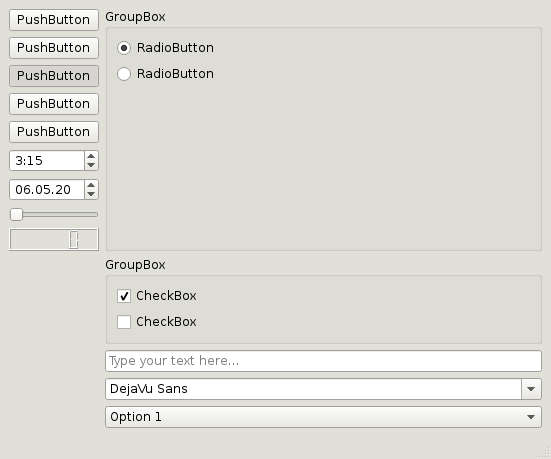
\includegraphics{graphics/laboratory/01-fusion.png}
\caption{Qt Fusion style example}\label{figure:fusion}
\end{figure}

\section{Getting and installing Qt}
There are basically three ways of obtaining Qt framework:
\begin{enumerate}
\item You have bought commercial Qt license so you can use specific Qt packages provided by Digia.
\item You can download open-source Qt framework directly from \href{http://www.qt-project.org/}{www.qt-pro\-/ject.org}.
\item You use a Linux distribution which can equip you with Qt framework via its packaging system.
\end{enumerate}

Qt can be downloaded as executable installer file which containes binaries precompiled for you as well as documentation and other needed tools. Sometimes manual compilation is needed.\footnote{It is commonly known that Qt compilation can last for several hours. Thus, consider getting precompiled binaries instead of compiling those by yourself.}

Precompiled Qt libraries are released for certain compilers only. Linux releases are should work with \fdocabbrevref{GCC}, Windows releases are usually precompiled by \fdocabbrevref{MSVC}. Qt framework with MinGW support is released from time to time too.

\subsection{Installing Qt on Windows}
Qt installation on Windows is fairly straightforward if precompiled Qt binaries are available. All you need to do is obtain the setup executable file and follow instructions. Some troubles might occur, though. Let's assume that Qt was installed in\fdocinlinecode{text}{!}{c:\\Qt\\Qt5.0.0\\}.

You need to change your PATH environment variable in order to be able to run Qt tools from command line. Qt Creator will work even without proper PATH because it does all necessary settings for itself automatically. You can setup PATH variable in Windows 7 as follows:
\begin{enumerate}
\item From the desktop, right-click (by mouse) \enquote{My Computer} and then click \enquote{Properties}.
\item Choose \enquote{Advanced System Settings} from the list.
\item In the \enquote{System Properties} window, hit the \enquote{Environment Variables} button.
\item Locate \enquote{System variables} group, select PATH variable and hit \enquote{Edit} button.
\item Move to the end of the string and add folowing paths:
\begin{lstlisting}[firstnumber=1,language=text]
c:\Qt\Qt5.0.0\5.0.0\msvc2010\bin\
c:\Qt\Qt5.0.0\Tools\QtCreator\bin\
\end{lstlisting}
Paths within the PATH variable are separated by semicolons. Typical content of PATH variable may look like the one in \autoref{listing:pathwindows}.
\begin{fdoccode}{text}{listing:pathwindows}{Setting PATH environment variable for Qt on Windows}
%SystemRoot%\system32;%SystemRoot%;c:\Qt\Qt5.0.0\5.0.0\msvc2010\bin\;c:\Qt\Qt5.0.0\Tools\QtCreator\bin\
\end{fdoccode}
\end{enumerate}

\subsection{Installing Qt on Linux}
As stated, Qt can be installed on Linux in two ways:
\begin{enumerate}
\item Linux distribution \textit{package manager}\index{package manager} offers it as the package. This is the case of many major distributions.
\item Classical installation via executable file:
\begin{enumerate}
\item Obtain installation file from \citep{various:qthome}.
\item Open terminal\index{terminal} and navigate to folder containing obtained installation file.
\item Change permissions on the file:
\begin{lstlisting}[firstnumber=1,language=text]
sudo chmod +x ./qt-5-installation-file.run
\end{lstlisting}
You need to run\fdocinlinecode{text}{!}{chmod} as superuser\index{superuser} (root\index{root}) if you want to install Qt into system-wide location.

\item Install Qt by executing\fdocinlinecode{text}{!}{./qt-5-installation-file.run}, follow on-screen instructions. It's good to install Qt into separate folder structure to keep system structure clean. Using\fdocinlinecode{text}{!}{/opt/qt5} as base installation directory is generally good idea.

\item There is no need of editing PATH environment variable if you use Qt Creator for development. Otherwise, make sure you set correct values to environment variables (see \autoref{listing:pathlinux}).
\begin{fdoccode}{text}{listing:pathlinux}{Setting environment variables for Qt on Linux}
QTDIR=/opt/qt5/5.0.0/gcc
PATH=$PATH:$QTDIR/bin
QMAKESPEC=$QTDIR/mkspecs/linux-g++
\end{fdoccode}
\fdocinlinecode{text}{!}{QTDIR} variable contains path to root qt directory. This is the directory which contains subdirectories\fdocinlinecode{text}{!}{bin},\fdocinlinecode{text}{!}{include},\fdocinlinecode{text}{!}{lib}, \ldots
\end{enumerate}
\end{enumerate}

\subsection{Compilling Qt}\index{compilation}
Sometimes, you may need to compile Qt on your own. Compilation allows you to throw away features you do not like, resulting in smaller dynamic/static libraries sizes.

Qt sources are always contained within compressed file. All you need to do is to have correctly installed \cpp{} compiler\footnote{Personally, I prefer \fdocabbrevref{GCC}-based compilers for Qt development.}. Basic compilation steps are quite similar for each operating system:
\begin{enumerate}
\item Decompress source package and navigate to its root folder using terminal (command prompt).
\item Run\fdocinlinecode{text}{!}{./configure -opensource -nomake examples -nomake tests}.
\item Now, run\fdocinlinecode{text}{!}{make} (on Linux),\fdocinlinecode{text}{!}{nmake} (on Windows with Visual Studio) or\fdocinlinecode{text}{!}{mingw32-make} (on Windows with MinGW).
\end{enumerate}

Compilation process can be complicated, as many problems can occur. See \citep{various:qtdoc} for more information.